\part*{Appendix}

\chapter{Installation, Setup and Settings}
\label{chap:installation}

\section{Back-end / Server}
\label{sec:backend-server}

In the following chapters the installation and setup of the back-end is described: The back-end uses Maven for its dependency management and build process. A local Tomcat server needs to be installed, the source code has to be downloaded from Github and the project needs to be configured as a Maven project.

\subsection{Installation}
To install Maven and build the system complete the following steps:

\begin{enumerate}
    \item Maven should be already integrated in Eclipse for JavaEE developers. If the following steps do not work, download and install maven and the m2e Eclipse plugin. During development, Eclipse Mars 4.5.1 was used.
    \item Clone or checkout the public reimbursement-server repository hosted on Github (see appendix \ref{github-source}).
    \item Import the project into Eclipse and then convert it to a Maven project.
    \item Run \texttt{mvn:install} to build and download all the dependencies required for the project.
    \item Download Apache Tomcat 8.0. Add the servers-view in Eclipse and click the link to create a new server. Create a new Tomcat server and add the reimbursement-server package to it.
    \item In the servers-view, double click the server-name and set the port of the Tomcat to 80 instead of 8080 and the startup timeout to approx. 90 seconds.
\end{enumerate}

\subsection{Server Settings}
In the settings section overall configuration parameters are defined and explained.

\subsubsection{LDAP}
\label{subsubsec:ldap}

Currently the synchronisation interval is set to 300 seconds. This value can be changed by adjusting the variable \textit{reimbursement.ldap.refreshRate} in the \texttt{application.properties} file that is stored in the back-end at \textit{src/main/resources} \par
During the development and integration a specific file will be loaded that defines the available demo user-accounts for the reimbursement-tool. Those users are defined in the file \texttt{development-server.ldif}. The following users exist:
\begin{itemize}
\item \texttt{junior} is a representative for the \textit{JuniorAssistants} group defined in the IFI LDAP tree.
\item \texttt{senior} is a representative for the \textit{SeniorAssistants} group defined in the IFI LDAP tree.
\item \texttt{prof} is a representative for the \textit{Professors} group defined in the IFI LDAP tree.
\item \texttt{fadmin} \& \texttt{fadmin2} are representatives for the \textit{Administration} group defined in the IFI LDAP tree.
\item \texttt{Depman} is a representative for the \textit{Departement Manager} defined in the IFI LDAP tree.
\item \texttt{Headinst} is a representative for the \textit{Head of Institute} defined in the IFI LDAP tree.

\end{itemize}

For all the demo user-accounts, the password is \textit{password}. To be able to login with the demo users, the test-ldap server has to run (is automatically started if the build profile is "DEV" or "INT") and also the demo-user SQL has to update the SQL Database (also done automatically in the "DEV" or "INT" profiles).

\subsubsection{E-mail server}
\label{subsubsec:email}

The e-mail settings can be adjusted in the \\ \texttt{application.properties} file in the back-end. To change the layout of an email, the corresponding email template has to be adapted. The email templates are stored in the directory \textit{src/main/resources/email}. To adjust an email template, we recommend to change the non-inlined version (\textit{src/main/resources/email/notInlinedTemplates}) and then inline it by using an inlining service like \textit{Ink.} (\url{http://foundation.zurb.com/emails/inliner.html}). To change the wording of the emails, the source texts in the "EmergencyEmailSendJob.java" and "NotificationSendJob.java" classes have to be adapted. These files are stored on the back-end in \textit{/src/main/java/ch/uzh/csg/reimbursement/model} folder. \newline \\
Some of the variables in the \texttt{application.properties} file depend on the maven profile and are therefore specified in the \texttt{pom.xml} file that is stored in the back-end's root folder.

\begin{lstlisting}
# If true this option stores an HTML
# file on the server instead of sending it to the email-receiver.
# the exact location can be seen in the email-log.
mail.redirectMailsToFile = ${mail.redirectMailsToFile}

# This crontrigger defines when the email are sent out
# http://www.quartz-scheduler.org)
mail.sendEmailsIntervalCron = ${mail.sendEmailsIntervalCron}
\end{lstlisting}

\subsubsection{Pdf Generation}
\label{subsubsec:pdf-xml-mappings}

The \textit{.xsl} file is used to generate an \textit{.fo} file out of an xml-file that consists of object data. In the folder \textit{src/main/resources} exists a \texttt{xml-mapping.xml} file that maps a data-object to a xml-object. The xml-object is required by the \texttt{xml2fo.xsl} and \texttt{attachmentXml2fo.xsl}. Those files transfer the xml-object into a \textit{.fo} file which is needed by the Apache FOP to generate the Pdf.



\section{Front-end / Client}

\subsection{Basic setup}
To run the front-end application on your local client, Node.js (incl. npm), Bower and Grunt need to be installed.

\paragraph{Node.js and Bower}
First we need to install Node.js (incl. npm) and Bower:
\begin{enumerate}
  \item Make sure, you have installed the latest version of Node.js. In development we used Node 5.4.0 and npm 3.3.12.
  \item Clone or checkout the public reimbursement-client repository hosted on Github (see appendix \ref{github-source}).
  \item Open a command-line tool and navigate to the root of the reimbursement-client directory and run \texttt{npm install}. This will download all required dependencies that are defied in the \textit{package.json}.
  \item While extensions to Node.js can be downloaded and installed by npm, the front-end dependencies like AngularJS, Flow.js and JQuery can conveniently be managed with Bower. If it is not already installed on your system (check in with \texttt{which bower}), install it by running \texttt{npm install -g bower}. After you have verified that Bower is installed run \texttt{bower install}. This will download all required dependencies that are defied in the \textit{bower.json}.
\end{enumerate}

\paragraph{Grunt}
Grunt builds the front-end files. It has multiple modules to build: you can concat, copy, prefix, sass-compile etc. The configuration of Grunt is stored in \textit{Gruntfile.js} and the modules grunt requires are loaded using npm.
\begin{enumerate}
  \item After all the steps in the npm section are completed, grunt needs to be installed. This can be done by \texttt{npm install -g grunt-cli}. Now we can start using the grunt CLI. There are various options available:
  \begin{itemize}
	\item \texttt{grunt}: This command starts the default grunt operation. It is used to build all the files. Use it only for development purpose, because the minified versions are not created.
	\item \texttt{grunt prod}: This command minifies and uglifies all the files. Use it to test if minification and uglification covers all the production requirements.
	\item \texttt{grunt serve}: This command starts a local http-server and updates automatically. If a source file is changed, the build will be executed and the browser will be reloaded to visualize the changes.
	\item \texttt{grunt prod-serve}: This command runs starts a local server with the production files as a base.
	\item \texttt{grunt deploy-int}: This command builds the project with the production profile and uploads the created files to the INTEGRATION Tomcat instance running on 192.41.136.227 (makes a redeploy). The deployment requires a deploy.json with the server configuration. Please refer to the Deployment section for details.
	\item \texttt{grunt deploy-prod}: This command builds the project with the production profile and uploads the created files to the PRODUCTION Tomcat instance running on 192.41.136.228 (makes a redeploy). The deployment requires a deploy.json with the server configuration. Please refer to the Deployment section for details.
    \end{itemize}
\end{enumerate}

\section{Deployment}

\subsection{Backend}

To deploy the software to the intergation or the production environment, the following steps are required:

\begin{itemize}
    \item Install maven. During development we used the JavaEE Eclipse as described in  \ref{sec:backend-server}.
    \item Store the credentials of the Tomcat instance and productive database in the maven directory. The hidden maven directory (\texttt{.m2}) is mostly stored inside the user's root directory. If there is no \texttt{.m2/settings.xml} file, create a new one. The file needs to have the following content:

    \begin{lstlisting}
    <settings xmlns="http://maven.apache.org/SETTINGS/1.0.0"
        xmlns:xsi="http://www.w3.org/2001/XMLSchema-instance"
        xsi:schemaLocation="
            http://maven.apache.org/SETTINGS/1.0.0
            http://maven.apache.org/xsd/settings-1.0.0.xsd">
    	<servers>
    		<server>
    			<id>reimbursement-server</id>
    			<username></username>
    			<password></password>
    		</server>
    	</servers>

    	<profiles>
    		<profile>
    			<id>reimbursement_int</id>
    			<properties>
    				<jdbc.username></jdbc.username>
    				<jdbc.password></jdbc.password>
    			</properties>
    		</profile>
    		<profile>
    			<id>reimbursement_prod</id>
    			<properties>
    				<jdbc.username></jdbc.username>
    				<jdbc.password></jdbc.password>
    			</properties>
    		</profile>
    	</profiles>
    </settings>
    \end{lstlisting}

    Add the respective user name and password values to login properly. Be aware, that the passwords need to be xml-encoded.

    \item To configure the deployment right click to the server project in Eclipse -> Run As -> Maven Build... and enter the following values in the corresponding input fields:
    \newline
    Name: \texttt{reimbursement-prod} or  \texttt{reimbursement-int}
    \newline
    Goals: \texttt{clean tomcat7:redeploy}
    \newline
    Profiles: \texttt{reimbursement\_prod} or \texttt{reimbursement\_int}
    \item run the new created maven build and the project will be deployed to the production/integration server.

\end{itemize}

Hint: If you do not enter the profile name here, the test database is started on your server and the H2 database is used.

\paragraph{Profiles}
There are currently three build profiles available \textit{reimbursement\_dev},  \textit{reimbursement\_int} and \textit{reimbursement\_prod}. Build profiles switch between the H2 database and the productive Postgres database. In the development and integration mode, additionally an LDAP server providing a few demo users to mock the real users is started. Additionally there are also inserted the same users into the database. \newline
By default, the profile \textit{reimbursement\_dev} is active. So an LDAP server is started and the H2 database is used. To enable the \textit{reimbursement\_prod} profile locally, pass the profile to the local tomcat. This can be achieved by right clicking on the project in the eclipse explorer | Properties | Maven and enter the word \textit{reimbursement\_dev} into the input field.

\paragraph{Clear PostgresDB}
\label{sec:clear-postgresdb}
To monitor the database version, Flyway is used. Flyway checks the database version and notifies about incompatible versions. This requires either to update the database version or to empty the existing database. To empty the existing PostgresDB without loosing database rights etc., a bashscript is available. To run the script, the VM needs to be accessed thru SSH and the script be run as root. The script is available in the directory \textit{/usr/share/tomcat7/reimbursement-database} named \textit{clear-postgres-database.bash}.

\subsection{Front-end}

\begin{itemize}

    \item Create a new file with the following content named \textit{deploy.json} in the root folder:
    \begin{lstlisting}
        {
            "username": "",
            "password": ""
        }
    \end{lstlisting}
    \item Add the credentials to the file. The deploy.json file has to be stored in the main directory.
    \item Open a command line tool and run \texttt{grunt deploy-int} or \texttt{grunt deploy-prod}. This will automatically deploy the front-end to the INT server or the PROD server. To modify the server's IP address, please refer to the \textit{grunt.js} file that is located in the client's root directory. 
    
\end{itemize}

\chapter{Models and Figures}

\section{Models}
\label{sec:app-models}

\begin{figure}[H]
    {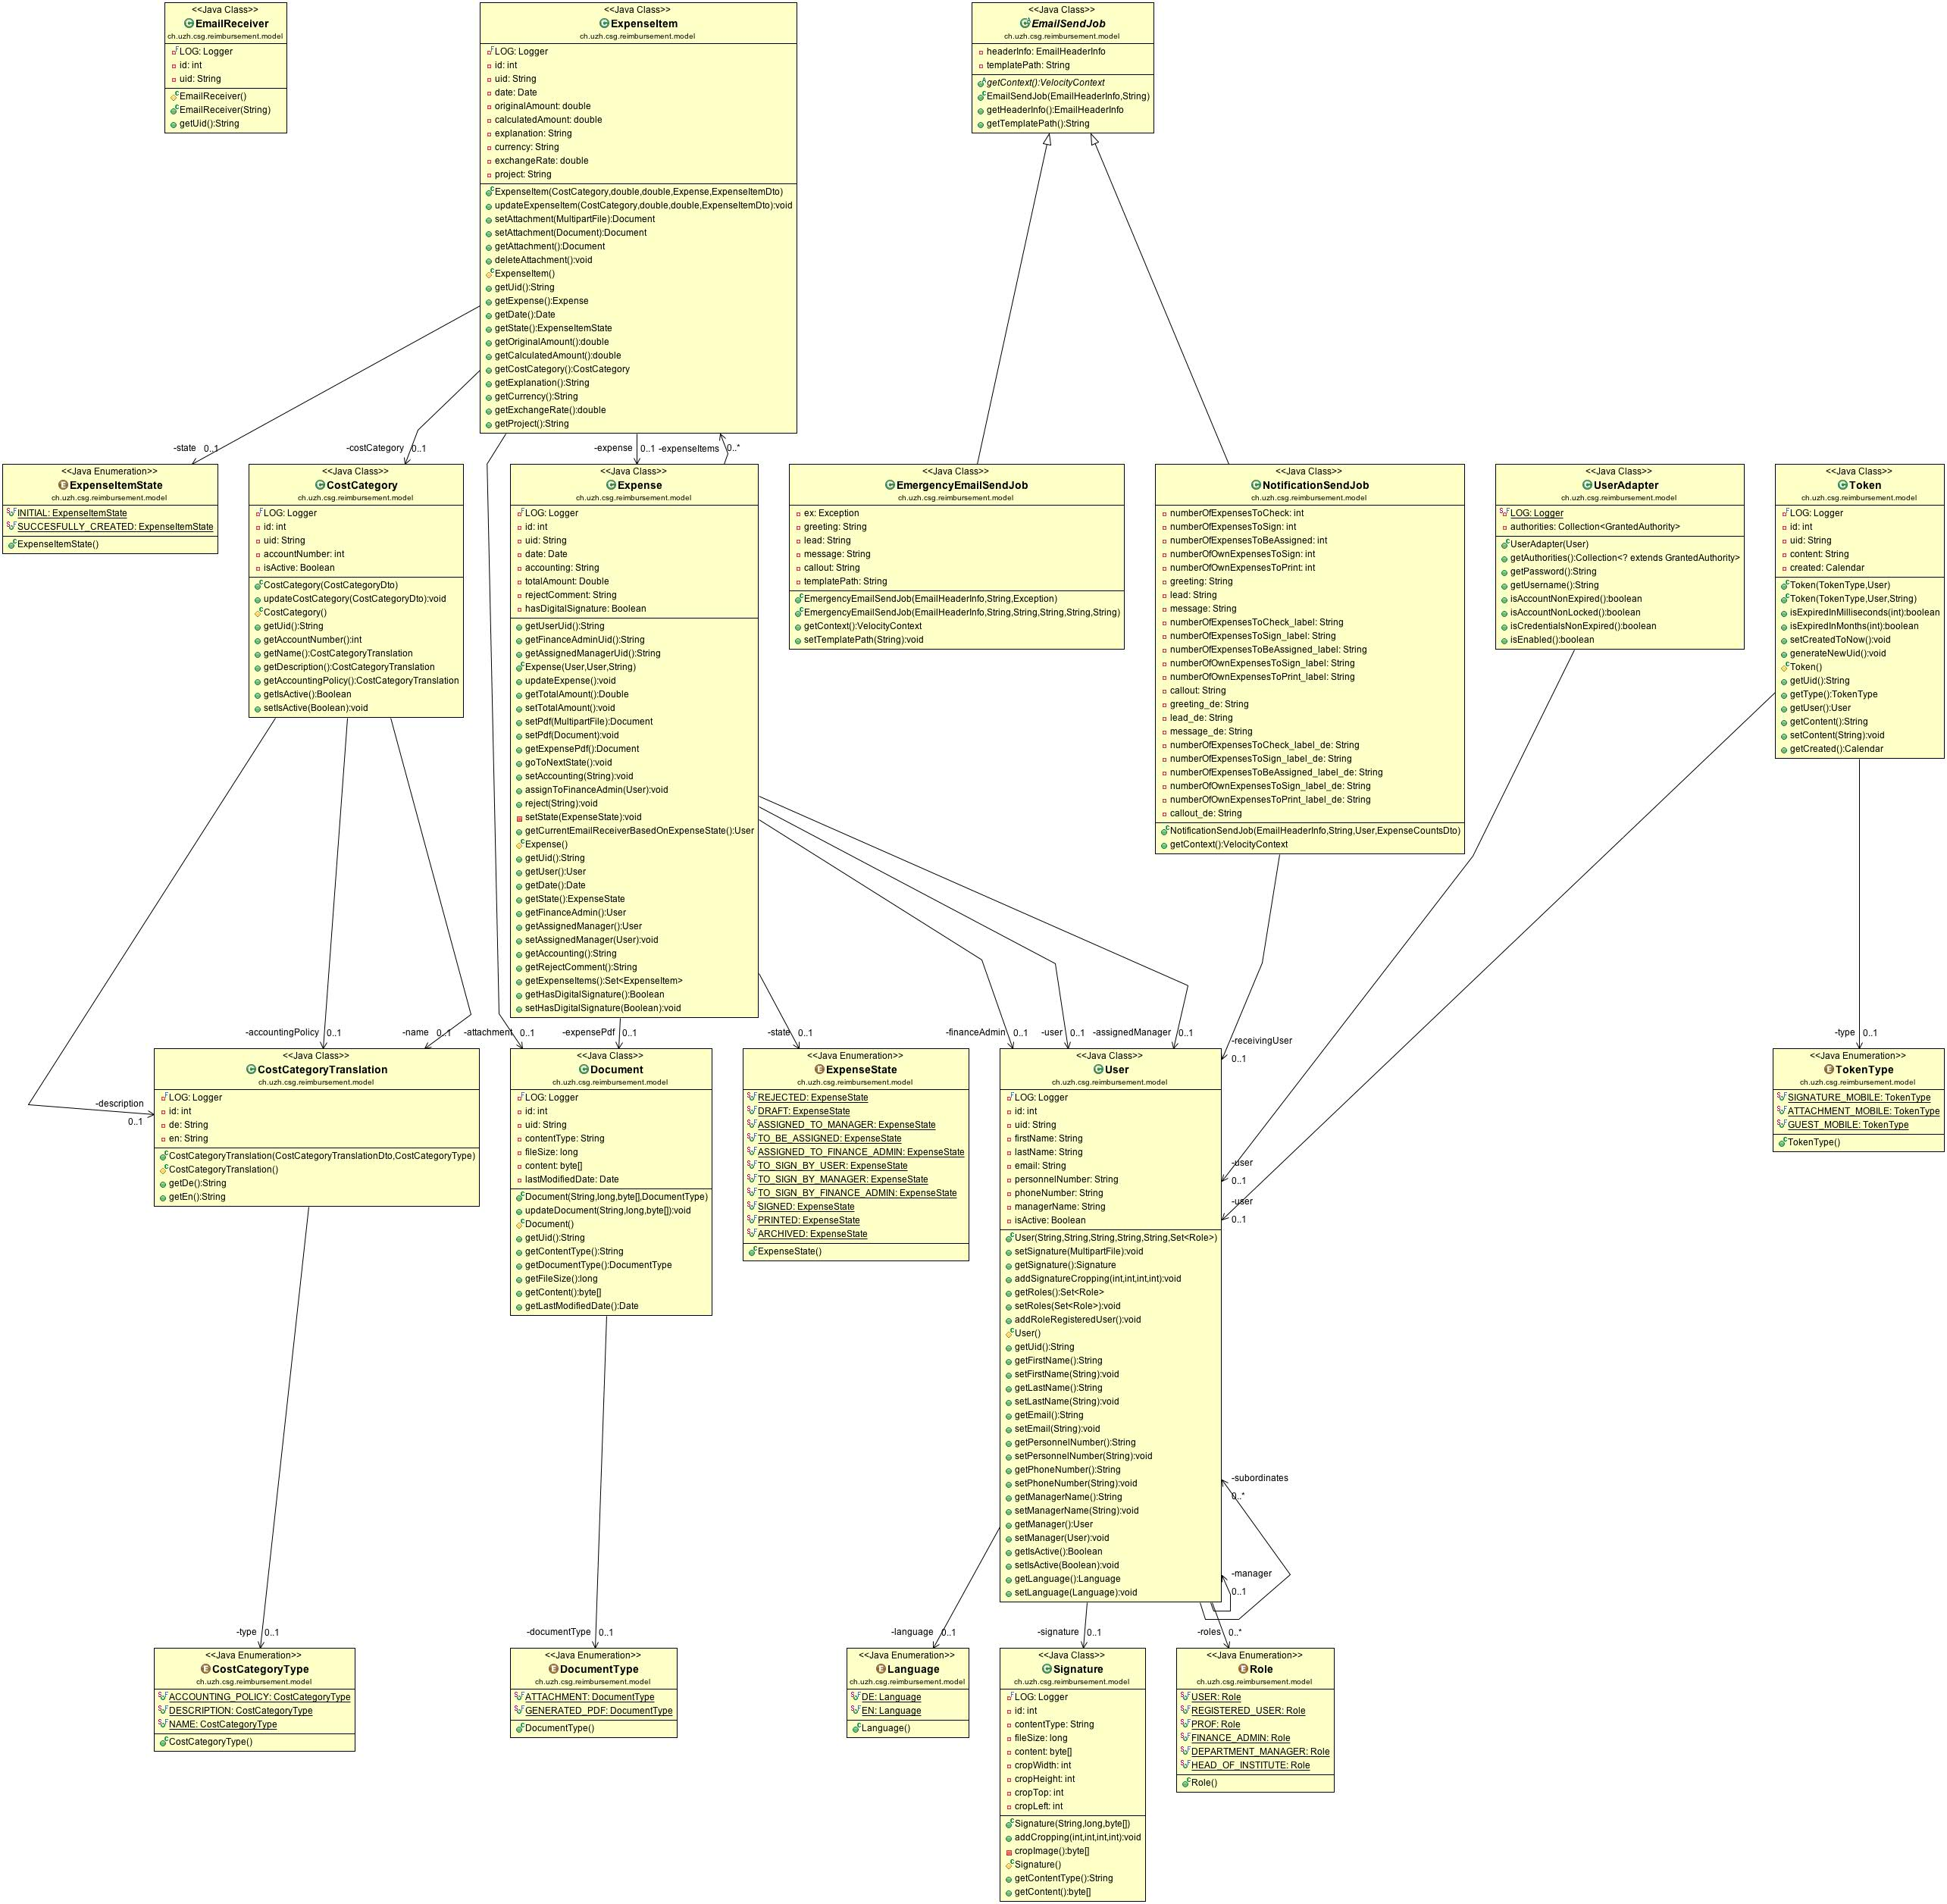
\includegraphics[width=1.0\textwidth]{umlclass-model}}
\end{figure}
\newpage

\section{Services}
\label{sec:app-service}

\begin{figure}[H]
    {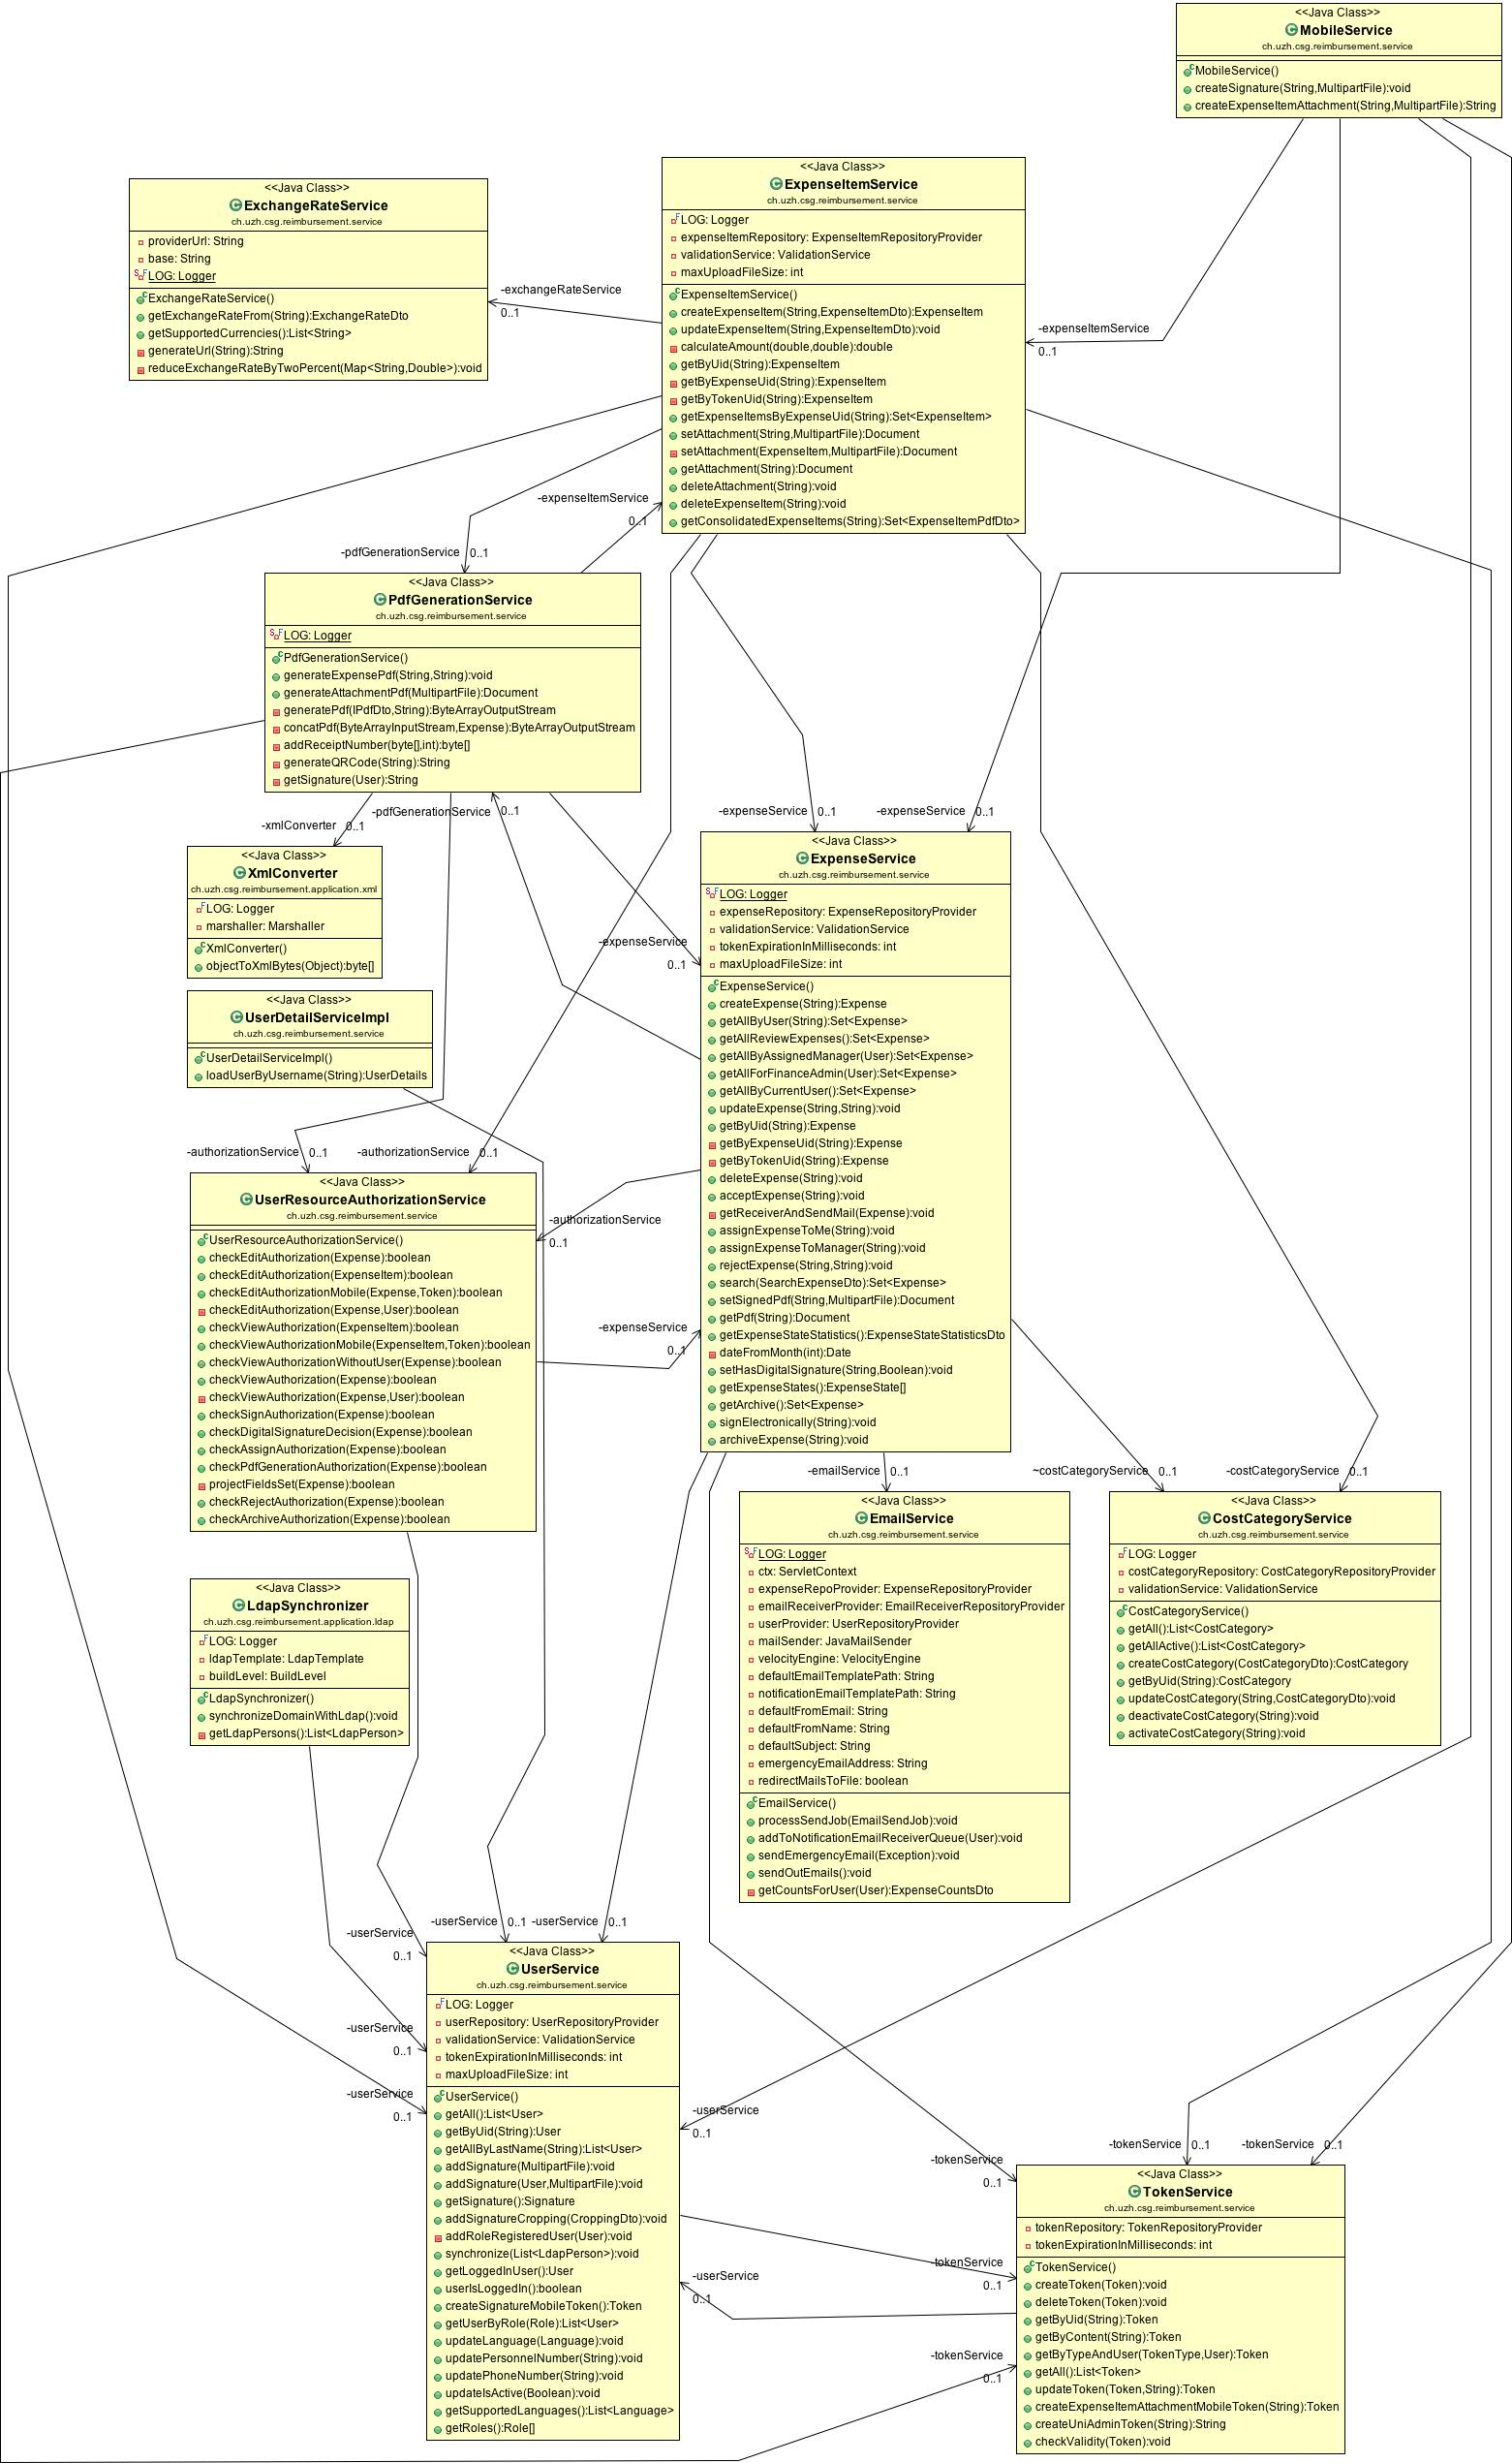
\includegraphics[width=0.8\textwidth]{umlclass-service}}
\end{figure}
\newpage

\section{REST Services}
\label{sec:rest-services}

\subsection{PRIVATE: expense services}
\begin{figure}[H]
    {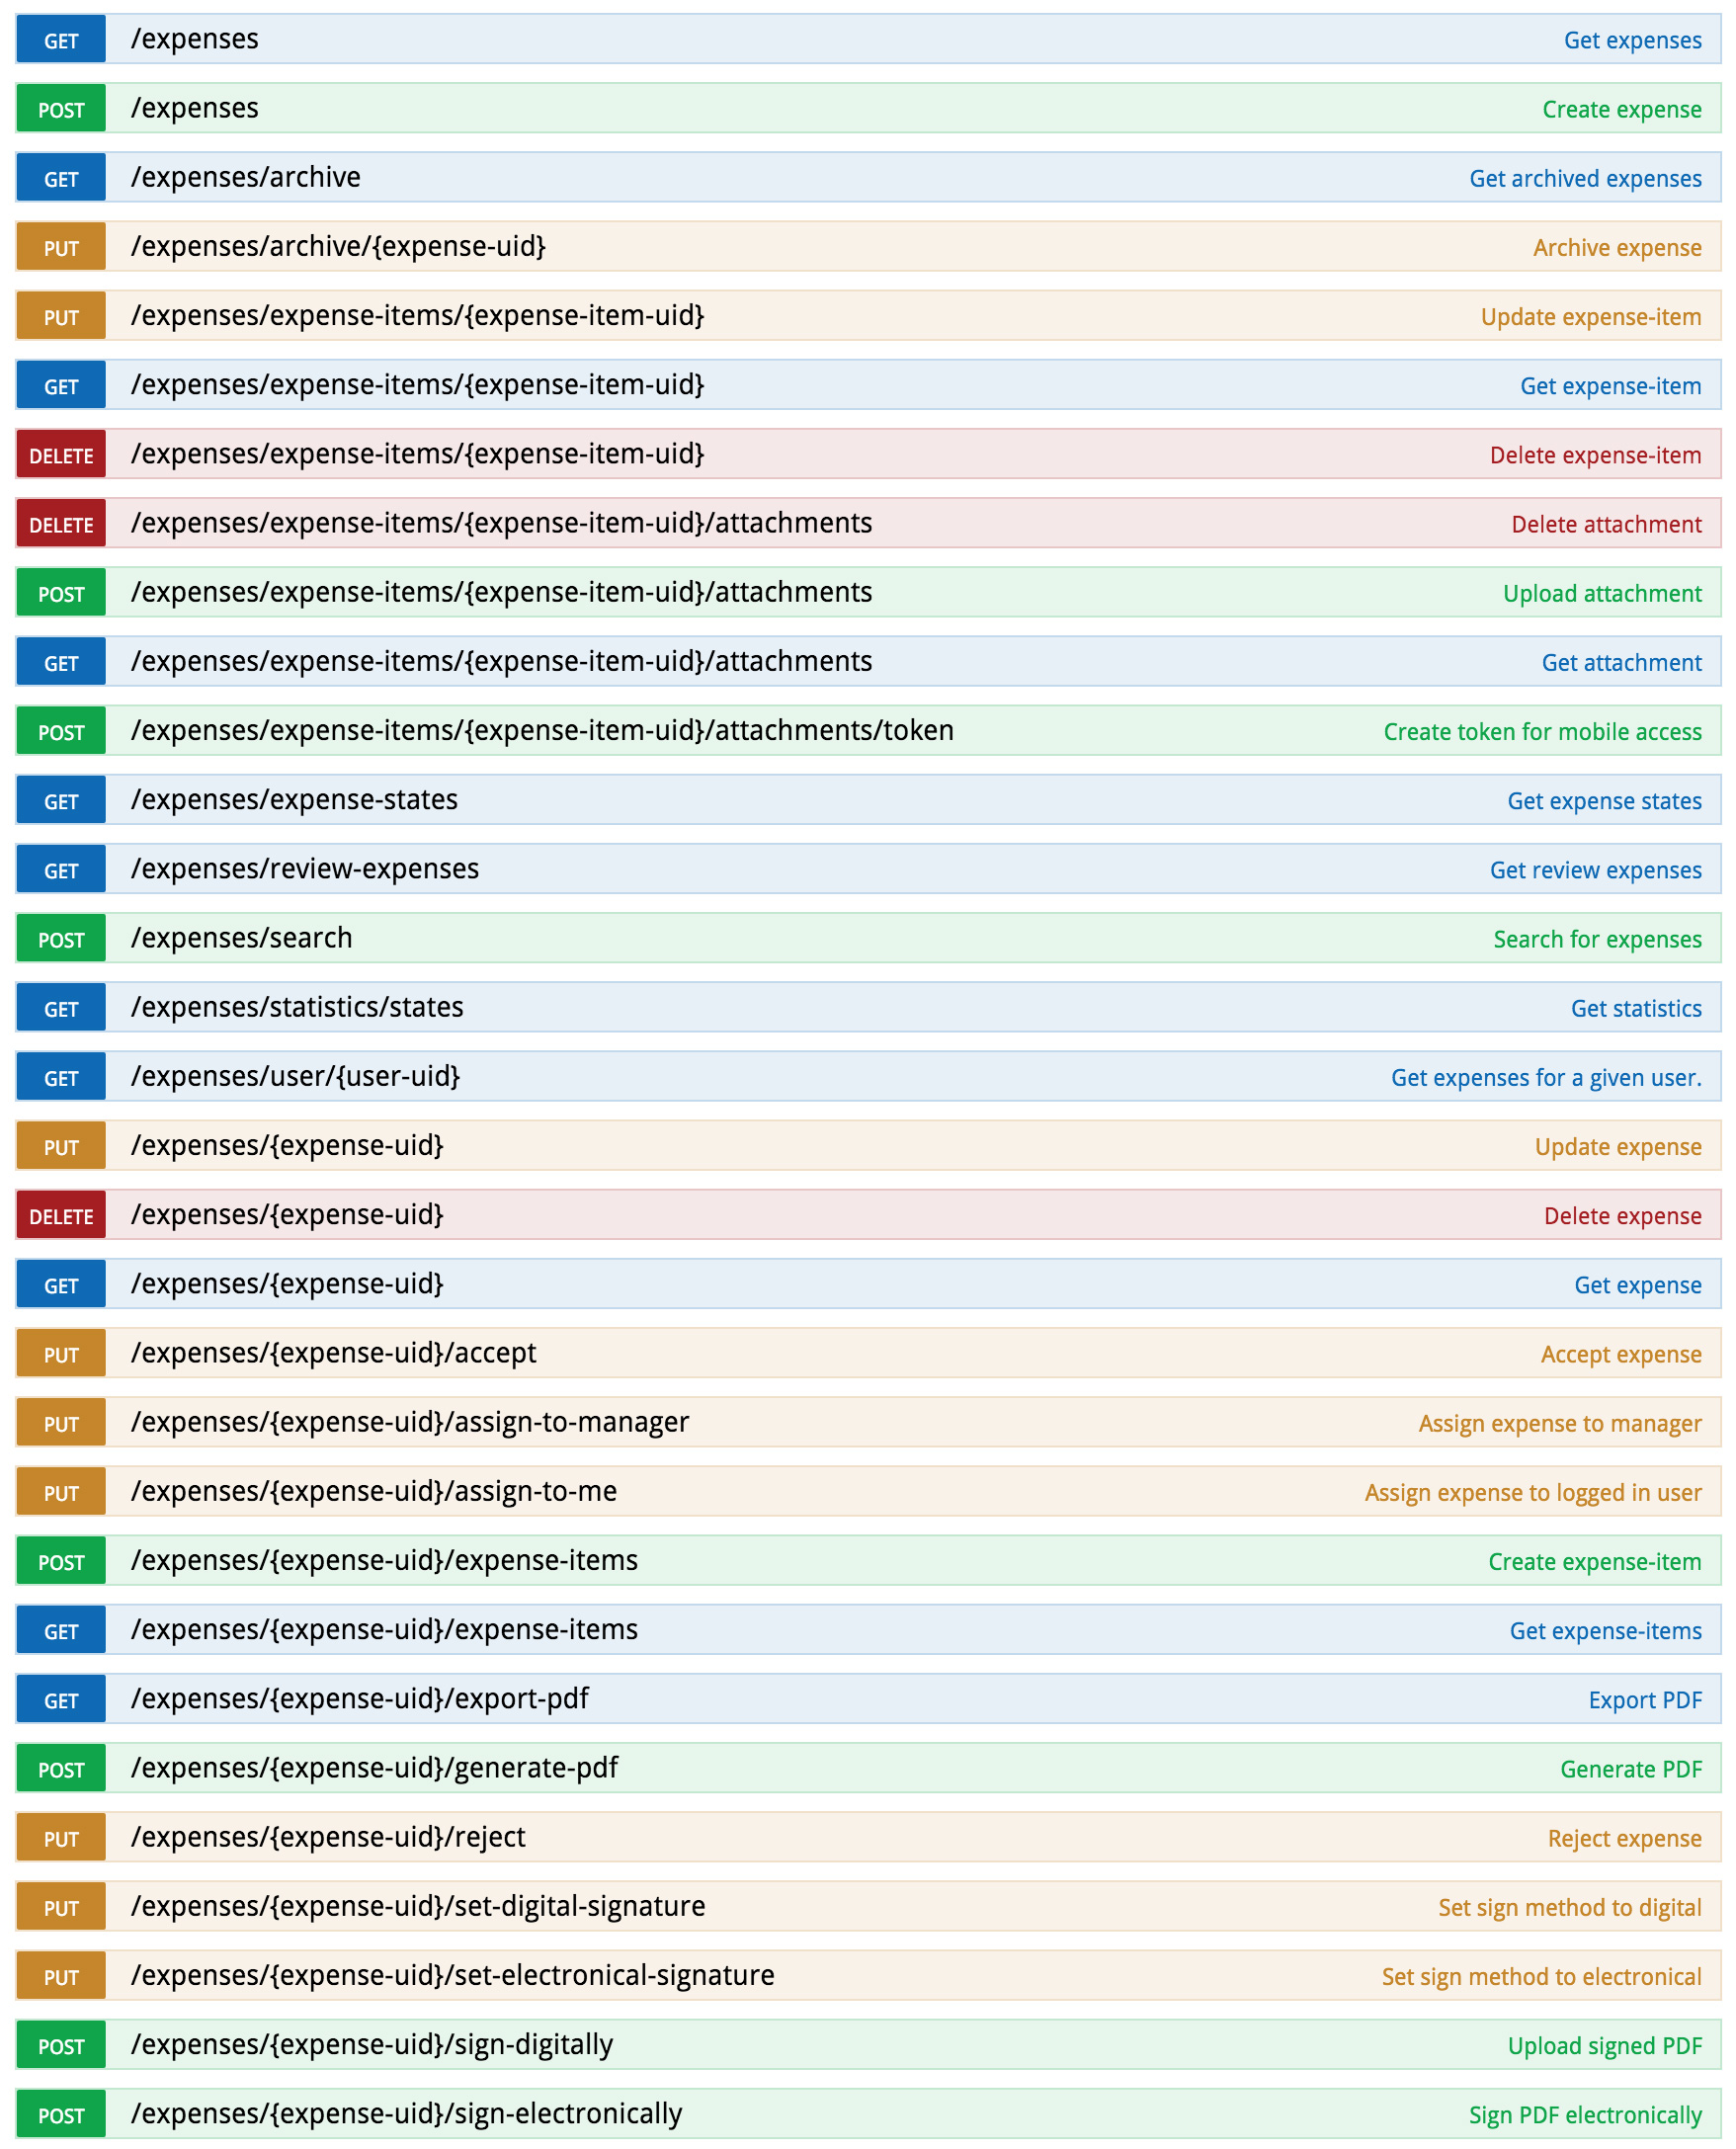
\includegraphics[width=0.95\textwidth]{rest-services_expense}}
\end{figure}
\newpage

\subsection{PRIVATE: finance administrator services}
\begin{figure}[H]
    {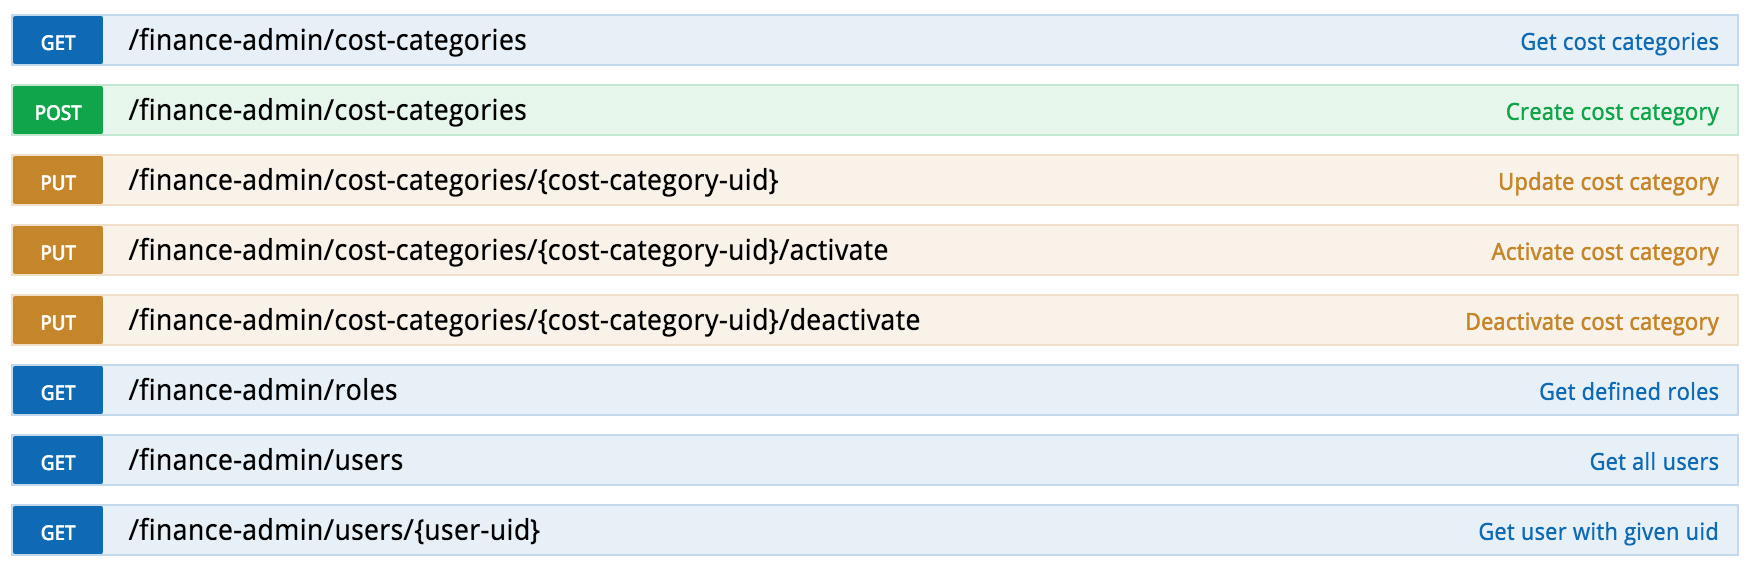
\includegraphics[width=0.95\textwidth]{rest-services_fa}}
\end{figure}

\subsection{PRIVATE: user services}
\begin{figure}[H]
    {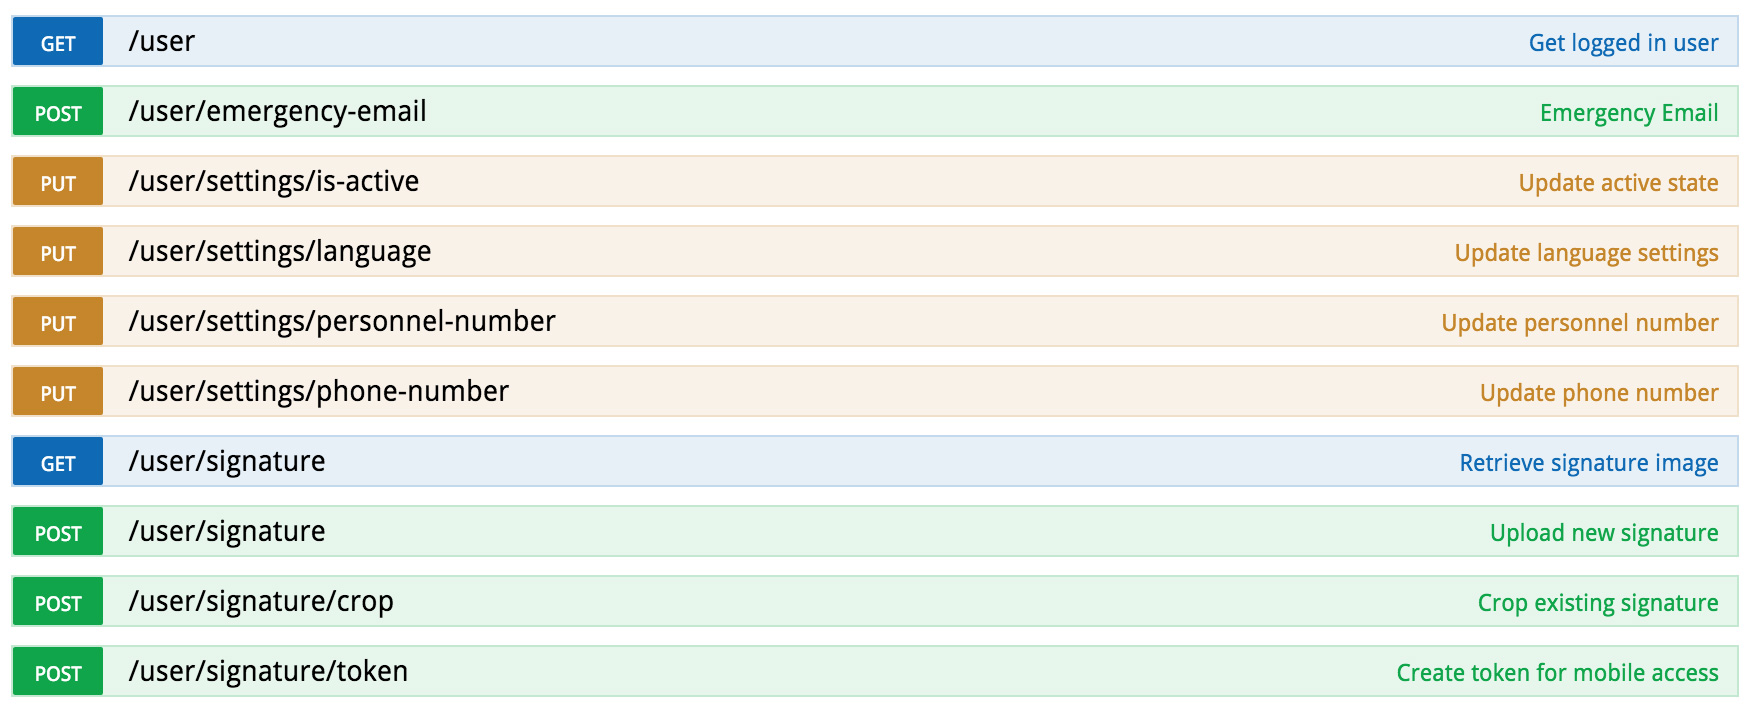
\includegraphics[width=0.95\textwidth]{rest-services_user}}
\end{figure}

\subsection{PUBLIC: various services}
\begin{figure}[H]
    {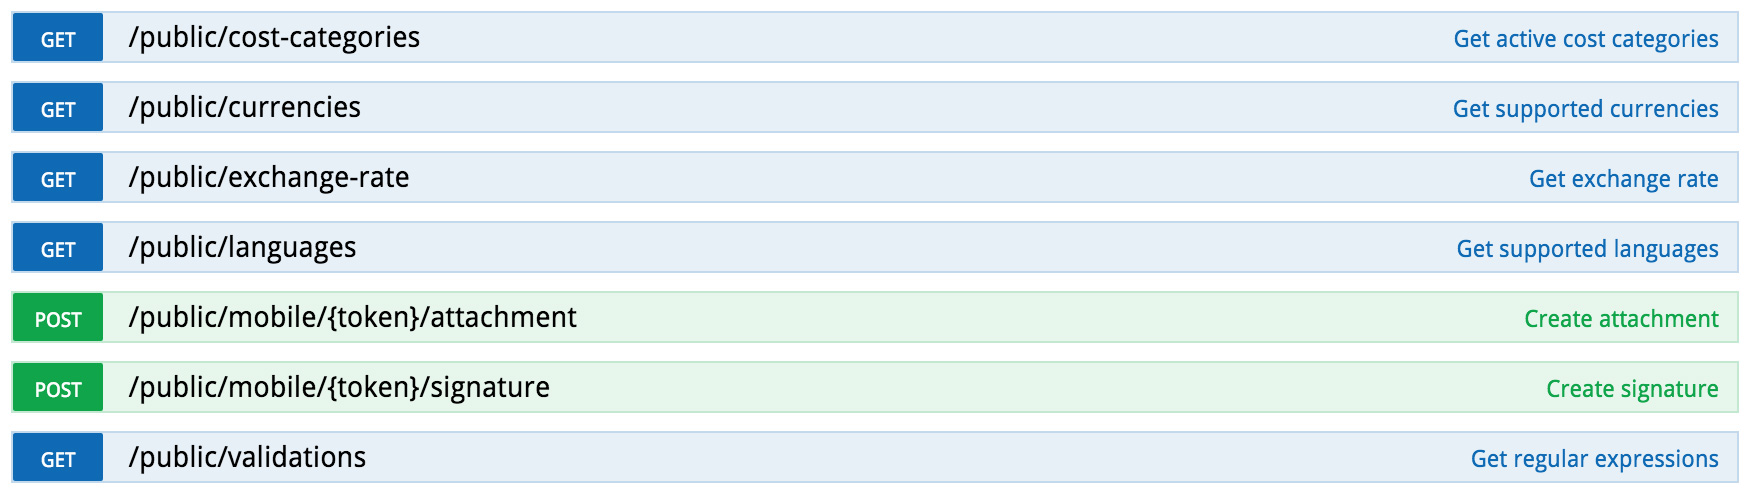
\includegraphics[width=0.95\textwidth]{rest-services_public}}
\end{figure}
\newpage

\section{Process diagram}
\label{sec:process-diagram-rotated}

\begin{figure}[H]
    {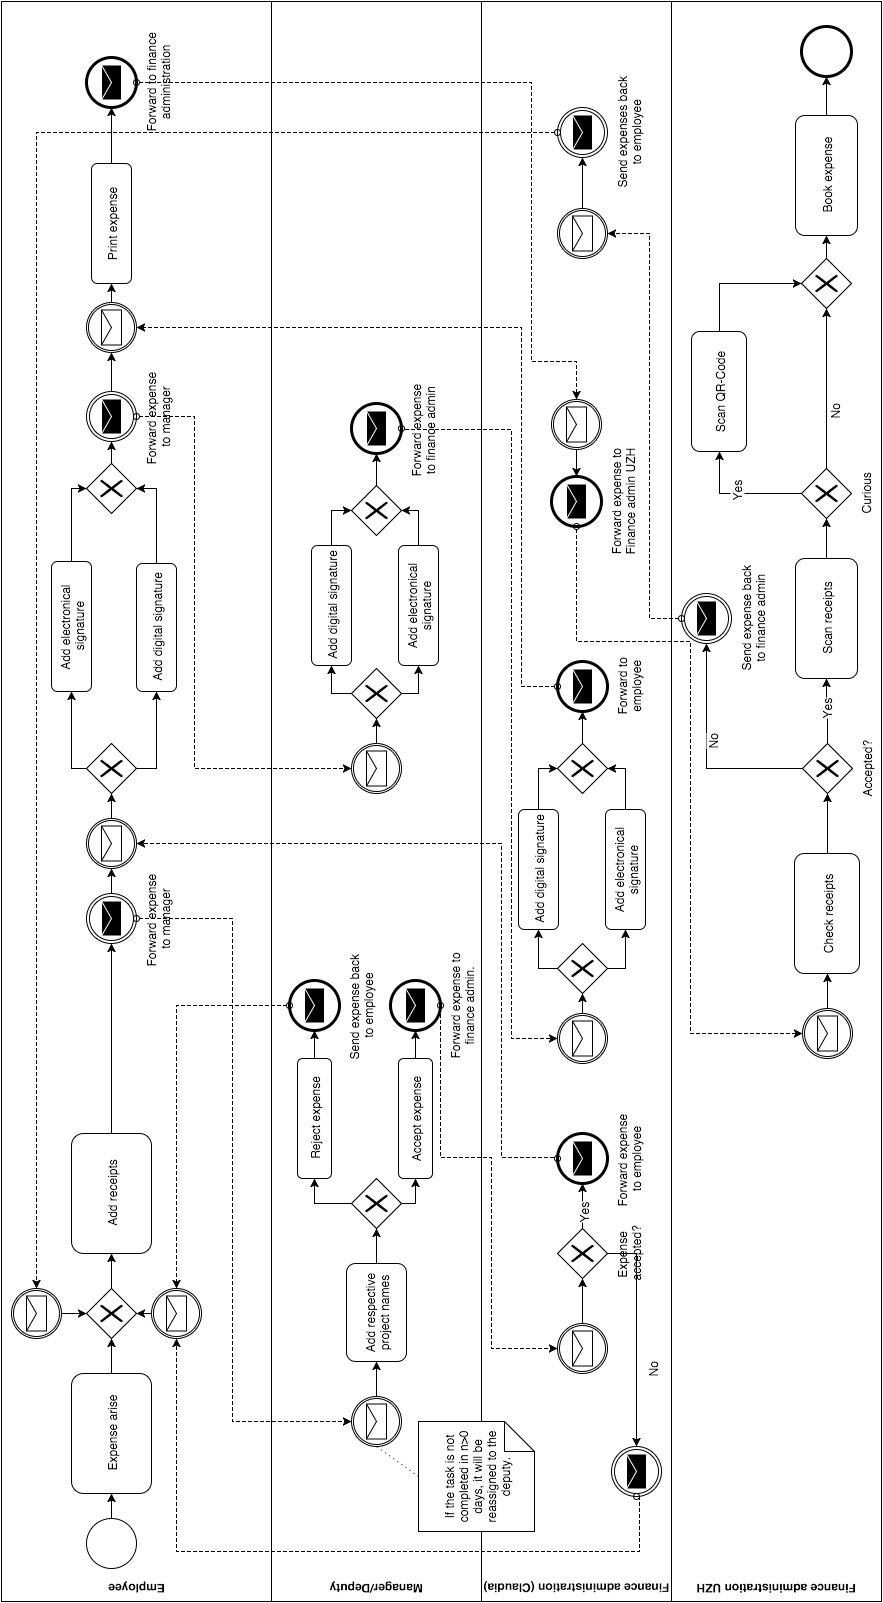
\includegraphics[width=0.75\textwidth]{process-diagram-rotated}}
\end{figure}
\newpage

\section{State diagram}
\label{sec:state-diagram}

\begin{figure}[H]
    {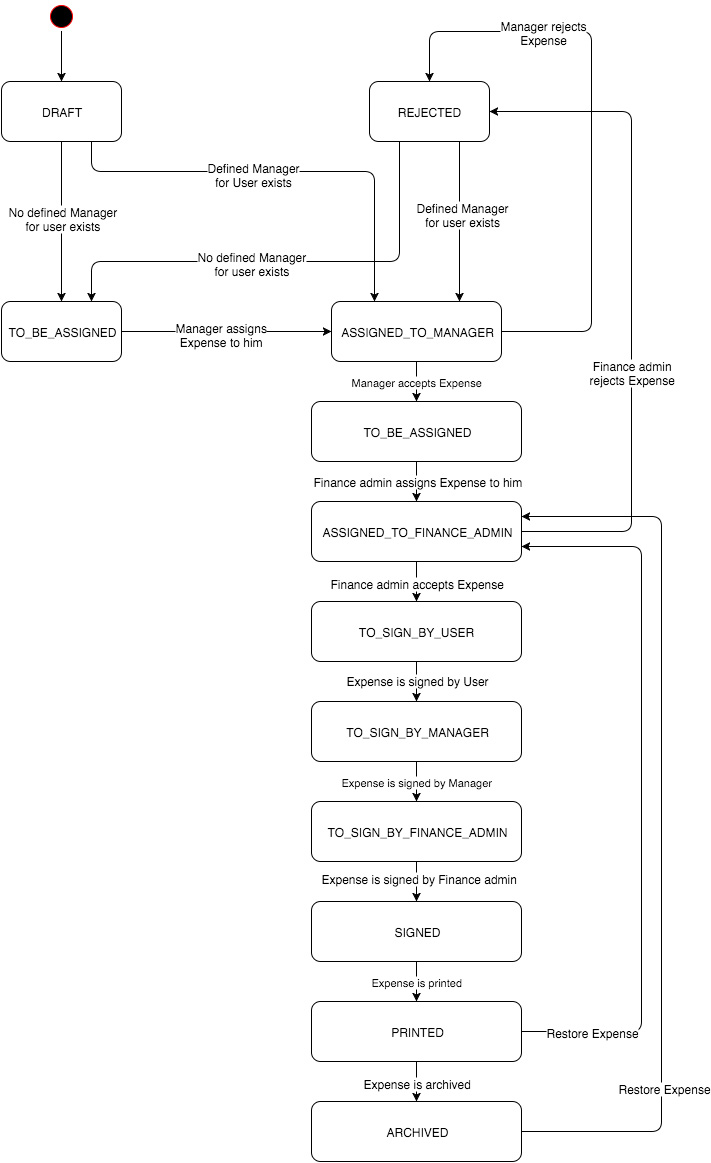
\includegraphics[width=0.8\textwidth]{state-diagram}}
\end{figure}
\newpage

\section{PDF}
\label{sec:app-pdf}

\begin{figure}[H]
    {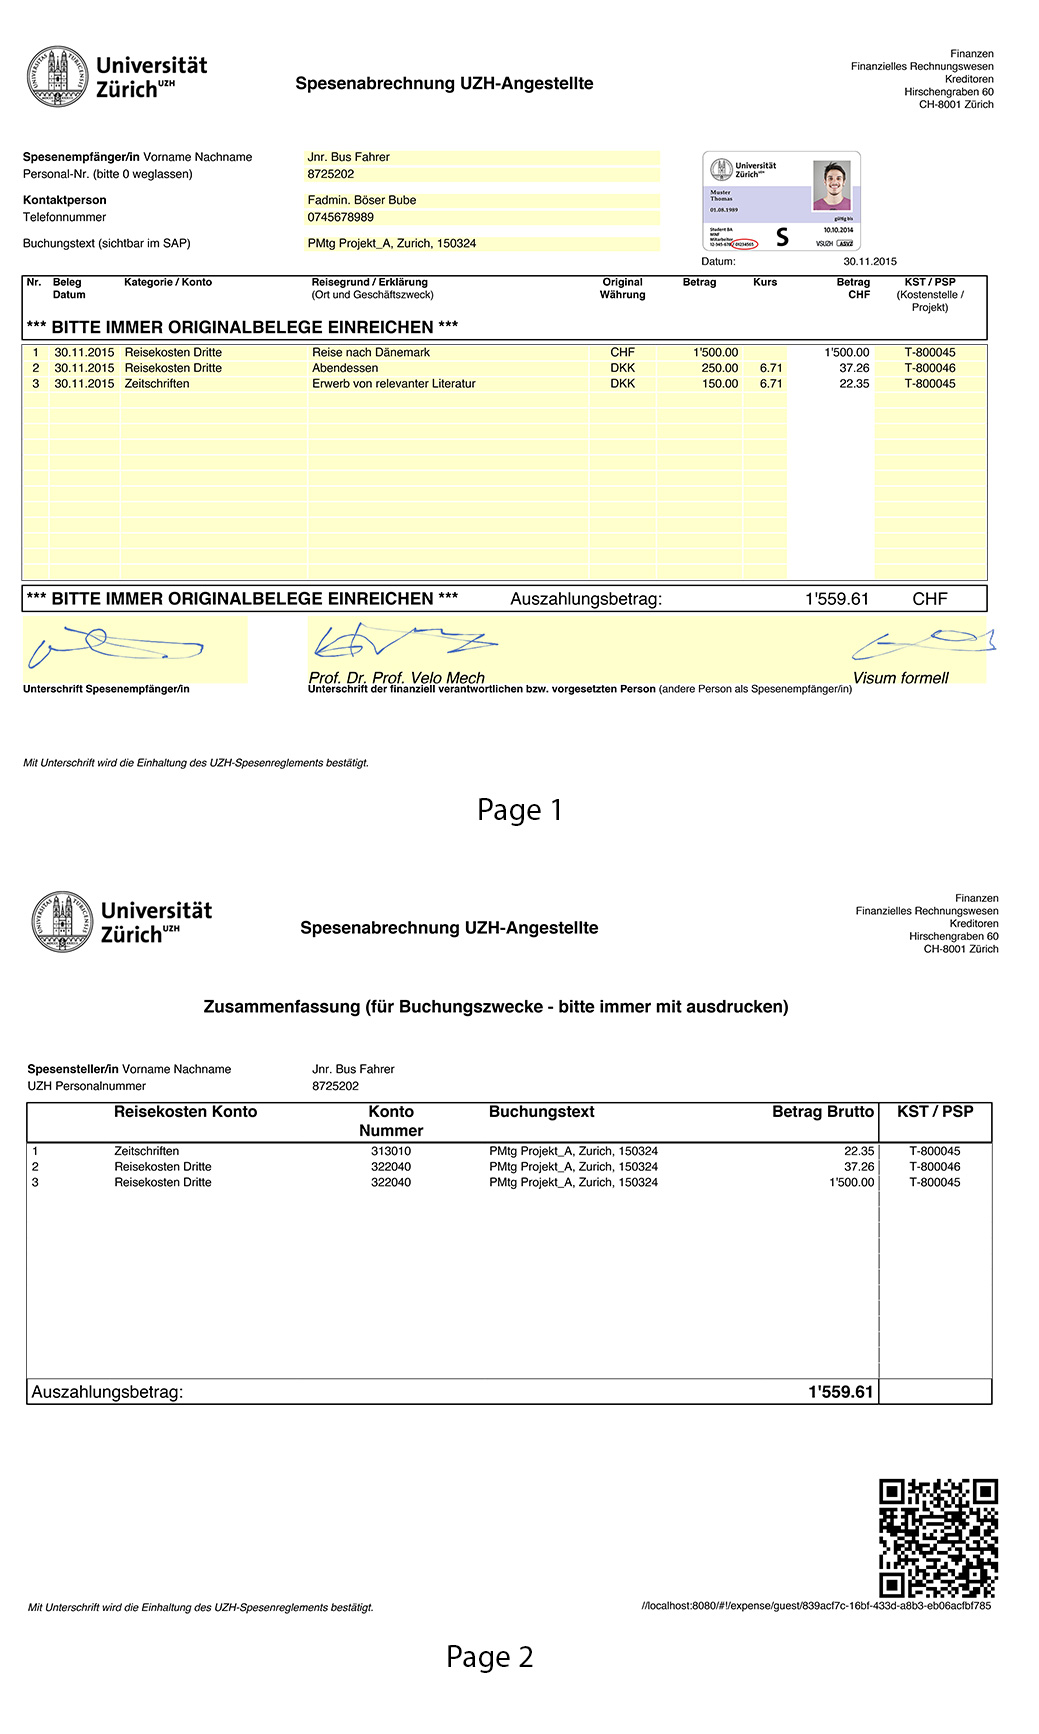
\includegraphics[width=0.8\textwidth]{pdf}}
\end{figure}
\newpage

\chapter{Software source-code}
\label{github-source}

The complete source code is available on a public repository on \url{http://github.com}. There exist four repositories: one for the front-end, one for the back-end, one for the technical documentation and one for the user manual.

\begin{itemize}
    \item Back-end: \newline \url{https://github.com/masterproject-reimbursement/reimbursement-server}
    \item Front-end: \newline \url{https://github.com/masterproject-reimbursement/reimbursement-client}
    \item Documentation: \newline \url{https://github.com/masterproject-reimbursement/reimbursement-documentation}
    \item User Manual: \newline \url{https://github.com/masterproject-reimbursement/reimbursement-manual}
\end{itemize}

For detailed installation instructions of the development environment and deployment steps, please refer to appendix \ref{chap:installation}.
